\documentclass[10pt]{article}
\usepackage{icmlko}

\icmlmeta{IP 파운데이션 월드모델}{249}{부분의 합이 아니다}{풀링 모형에서 부호화 변경은 도메인에 나눠 붙일 수 없다 --- 교차항이 부분합만큼 크다}

\begin{document}

\twocolumn[
\icmlheader

\begin{abstract}
노트 248이 남긴 제일 큰 항목 --- 게임이 도메인 안 백분위 정규화로
$-$0.084($t{=}-2.31$)를 잃는다, 왜인가. 손 축 다섯을 하나씩 정규화해 봤는데
\textbf{어느 하나도 그 값을 못 만든다}(제일 큰 것이 \texttt{media\_push}
$-$0.038, $t{=}-1.57$). 그래서 갈래를 바꿔 \emph{누가} 바뀌는지로 갈랐다.
\textbf{게임만 정규화하면 $-$0.0125($t{=}-0.72$)}, \textbf{게임 빼고 나머지
여덟만 정규화하면 $-$0.0164($t{=}-1.36$)}. 둘 다 유의하지 않고 합쳐도
$-$0.029 다. 그런데 둘 다 하면 $-$0.084($t{=}-2.33$)다 --- \textbf{교차항이
$-$0.055 로 부분합의 두 배}다. 게임만의 일인지 보려고 큰 도메인 다섯에 다
했다. \textbf{일반이다}: $\sum|$교차항$| = 0.091$ 이고 $\sum|$부분합$| =
0.093$ 으로 \textbf{비가 0.98}, 절반이 교차항이다. 웹툰은 \textbf{부호까지
갈린다} --- 자기가 바꾸면 $-$0.020 인데 남이 바꾸면 $+$0.035 다. 뜻은
날카롭다. 풀링 모형에서 \textbf{부호화 변경의 손익은 도메인에 나눠 붙일 수
없다.} 노트 246은 ``자료를 고친 곳이 아니라 남이 치른다''를 봤는데, 이제
한 걸음 더 간다 --- \textbf{어느 쪽도 치르지 않는다. 치르는 것은 둘 사이다.}
따라서 ``이 도메인 부호화를 고치면 그 도메인이 얼마 얻나''는 \emph{원리적으로}
답이 없는 질문이고, 도메인별 A/B 로 부호화를 고르는 절차는 전부 무효다.
\end{abstract}
]

\section{축으로는 안 갈라진다}

노트 247이 손 축 다섯을 도메인 안 백분위로 맞췄을 때 게임이 $-$0.084 를
잃었고, 노트 248이 그것을 $|t| \ge 2$ 인 진짜 효과 둘 중 하나로 확인했다.
먼저 축을 하나씩 정규화해 봤다.

\begin{center}\small
\begin{tabular}{lrr}
\hline
정규화한 축 & 게임 & $t$ \\
\hline
\texttt{media\_push} & $-$0.0378 & $-$1.57 \\
\texttt{target\_breadth} & $-$0.0105 & $-$0.61 \\
\texttt{goods\_scale} & $-$0.0068 & $-$0.90 \\
\texttt{entry\_friction} & $-$0.0024 & $-$0.50 \\
\texttt{venue\_prominence} & $-$0.0005 & $-$0.14 \\
\hline
\textbf{다섯 다} & $\mathbf{-0.0840}$ & $\mathbf{-2.33}$ \\
\hline
\end{tabular}
\end{center}

다섯을 더해도 $-$0.058 이고, 유의한 것은 하나도 없다. 축이 답이 아니다.

여기서 눈에 걸리는 것이 하나 있었다. 게임은 손 축 값이 제일 \emph{많은}
도메인이다.

\begin{center}\small
\begin{tabular}{lrrrr}
\hline
서로 다른 값 & 게임 & 웹툰 & 애니 & 모바일 \\
\hline
\texttt{target\_breadth} & \textbf{111} & 12 & 5 & 30 \\
\texttt{media\_push} & \textbf{177} & --- & 3 & 17 \\
\texttt{goods\_scale} & 96 & 308 & --- & 1784 \\
\hline
\end{tabular}
\end{center}

값이 111개면 도메인 안 백분위는 사실상 단조 재척도일 뿐이라 \emph{안에서는}
순서가 하나도 안 바뀐다. 그런데 제일 많이 잃는다. 그러면 손해는 게임 안에
없다.

\section{누가 바뀌는지로 갈랐다}

\begin{figure}[t]
\centering
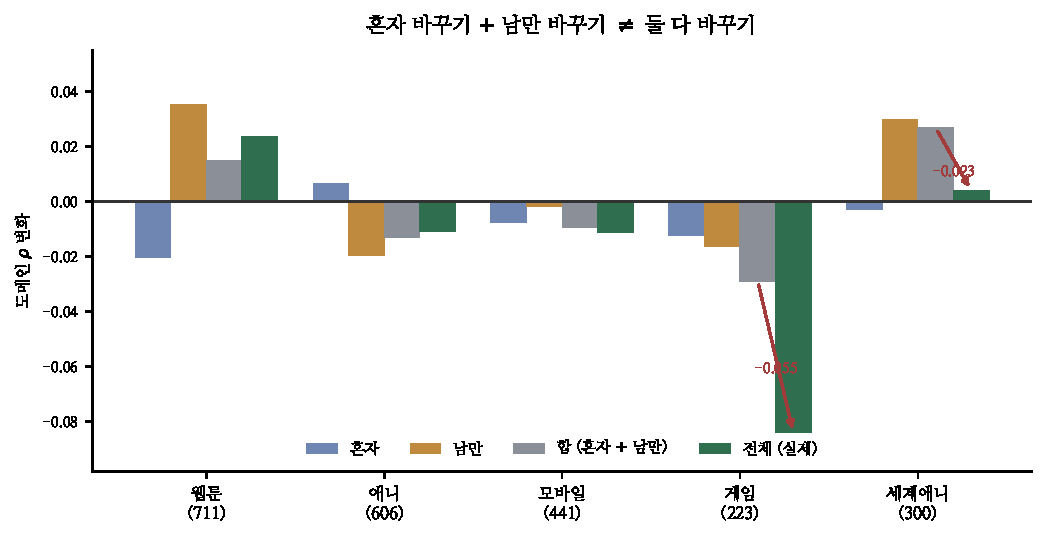
\includegraphics[width=\columnwidth]{figs/parts.pdf}
\caption{도메인마다 ``혼자 바꿈'' · ``남만 바꿈'' · 그 합 · 실제. 빨간
화살표가 교차항이다.}
\end{figure}

\begin{center}\small
\begin{tabular}{lrr}
\hline
무엇을 정규화 & 게임 & $t$ \\
\hline
게임만 & $-$0.0125 & $-$0.72 \\
게임 빼고 여덟만 & $-$0.0164 & $-$1.36 \\
\hline
합 & $-$0.0289 & \\
\textbf{둘 다} & $\mathbf{-0.0840}$ & $\mathbf{-2.33}$ \\
\textbf{교차항} & $\mathbf{-0.0551}$ & \\
\hline
\end{tabular}
\end{center}

\textbf{어느 쪽도 혼자서는 유의하지 않은데 둘 다 하면 유의하다.} 예측
순위상관으로도 같다 --- 게임만 바꾸면 예측이 $+$0.956 으로 거의 그대로고,
남만 바꿔도 $+$0.978 인데, 둘 다 하면 $+$0.836 으로 무너진다.

기전은 풀링의 구조 그 자체다. 손 축 계수는 아홉 도메인이 공유하므로,
남들이 바뀌면 계수가 새로 맞춰지고 게임은 \emph{옛} 값으로 그 계수를 받는다
(그래도 견딜 만하다). 게임만 바뀌면 계수는 거의 그대로인데 게임 값이 새것이
된다(역시 견딜 만하다). 둘 다 바뀌면 \textbf{새 계수와 새 값이 서로 안 맞는
방향으로 동시에 움직인다.}

\section{게임만의 일이 아니다}

\begin{figure}[t]
\centering

\includegraphics[width=\columnwidth]{figs/ratio.pdf}
\caption{다섯 도메인. 점선 위면 교차항이 부분합보다 크다.}
\end{figure}

\begin{center}\small
\begin{tabular}{lrrrr}
\hline
도메인 & 혼자 & 남만 & 합 & 교차항 \\
\hline
웹툰 & $\mathbf{-0.020}$ & $\mathbf{+0.035}$ & $+$0.015 & $+$0.009 \\
애니 & $+$0.007 & $-$0.020 & $-$0.013 & $+$0.002 \\
모바일 & $-$0.008 & $-$0.002 & $-$0.010 & $-$0.002 \\
게임 & $-$0.013 & $-$0.016 & $-$0.029 & $\mathbf{-0.055}$ \\
세계애니 & $-$0.003 & $+$0.030 & $+$0.027 & $\mathbf{-0.023}$ \\
\hline
\end{tabular}
\end{center}

\[ \sum |{\rm 교차항}| = 0.091, \qquad \sum |{\rm 부분합}| = 0.093. \]

\textbf{비가 0.98 --- 절반이 교차항이다.} 그리고 웹툰은 부호가 갈린다:
\textbf{자기가 바꾸면 잃고($-$0.020) 남이 바꾸면 얻는다($+$0.035).}
세계애니는 남이 바꿔 준 $+$0.030 을 교차항 $-$0.023 이 거의 다 도로
가져간다.

\section{답이 없는 질문}

이 실험실이 지금까지 부호화를 두고 물어 온 형태는 이랬다 --- ``모바일
가격 눈금을 고치면 모바일이 얼마 얻나''(노트 246), ``웹툰 태그 경계를
넓히면 웹툰이 얼마 얻나''(노트 240). \textbf{그 질문에는 답이 없다.}
손익의 절반이 그 도메인에도 남에게도 안 붙고 \emph{둘 사이}에 있기 때문이다.

노트 246은 ``자료를 고친 곳이 아니라 남이 치른다''로 한 걸음 갔다. 여기가
그 다음 걸음이다 --- \textbf{어느 쪽도 치르지 않는다.} $-$0.084 중
$-$0.013 만 게임이, $-$0.016 만 남이 내고, 나머지 $-$0.055 는 \emph{짝}이
낸다.

곧바로 따라오는 것: 도메인별 A/B 로 부호화를 고르는 절차는 전부 무효다.
게임 부호화를 게임에서만 시험하면 $-$0.013($t{=}-0.72$)이라 ``차이 없음''이
나오고, 그 규약을 전 도메인에 배포하는 순간 $-$0.084 가 된다. \textbf{6배
틀린다.}

\section{그러면 무엇을 하나}

부호화는 \textbf{전 도메인 동시 변경으로만} 재고, 판정은 판 $\rho$ 와
\texttt{rank.spread} 의 ``진짜 총량''을 나란히 본다(노트 247 · 248). 그것이
지금 우리가 할 수 있는 전부다 --- 그리고 노트 247이 이미 그렇게 재서
``판으로는 정할 수 없다''는 답을 얻었다. 이 노트는 그 답을 못 뒤집지만
\textbf{왜 정할 수 없는지}를 준다. 도메인별로 뜯어서 정하고 싶었는데,
뜯을 수 없는 것이었다.

\paragraph{남은 것}
\begin{center}\small
\begin{tabular}{ll}
\hline
갈래 & 왜 \\
\hline
웹툰 부호 갈림 & 남이 바꾸면 $+$0.035. 남의 부호화가 웹툰 자산이다 \\
교차항 예측 & 라벨 없이 어림할 길이 있나(분포 겹침?) \\
\texttt{by\_kind} & 선호형/양형도 SE 없이 보고한다(노트 248) \\
도메인별 A/B & 부호화 말고 \emph{축 추가}도 같은 병인가 \\
\hline
\end{tabular}
\end{center}

\paragraph{규약} \textbf{부호화 변경은 도메인별로 시험하지 않는다.} 한
도메인에서 재면 교차항이 빠져 평균 절반, 게임의 경우 6분의 1 로 작게
나온다. 전 도메인 동시 변경으로만 재고, 그렇게 재도 판정은 대개 못 한다.

\end{document}
